\setcounter{section}{2}
\section{Đường thẳng song song với mặt phẳng}
\subsection{Tóm tắt lý thuyết}
\begin{tomtat}
\subsubsection{Đường thẳng song song với mặt phẳng}
\begin{dn}
	Đường thẳng được gọi là song song với mặt phẳng nếu chúng không có điểm chung.
\end{dn}
\subsubsection{Điều kiện và tính chất}
\begin{dl}[dấu hiệu nhận biết một đường thẳng song song với một mặt phẳng]
	\immini
	{
	Nếu đường thẳng $a$ không nằm trong mặt phẳng $(P)$ và $a$ song song với đường thẳng $a'$ nằm trong $(P)$ thì $a$ song song với $(P)$.
	}
	{
	\begin{tikzpicture}[scale=1, font=\footnotesize, line join=round, line cap=round, >=stealth]
	\path
	(0,0) coordinate (A)
	(4,0) coordinate (B)
	(3,-1.5) coordinate (C)
	($(A)+(C)-(B)$) coordinate (D)
	(0,1.5) coordinate (E)
	(3.5,1.5) coordinate (F)
	(0,-0.5) coordinate (G)
	(3.5,-0.5) coordinate (H)
	;
	\draw (E)--(F)node[above]{$a$}
	(G)--(H)node[above]{$a'$} (A)--(B)--(C)--(D)--(A)
	;
	\draw pic["$(P)$", draw=black, angle eccentricity=0.65, angle radius=0.7cm]{angle=C--D--A};
	\end{tikzpicture}
	}
\end{dl}
\begin{dl}[Tính chất của đường thẳng song song với mặt phẳng]
	Cho đường thẳng $a$ song song với mặt phẳng $(P)$. Nếu mặt phẳng $(Q)$ chứa $a$ và cắt $(P)$ theo giao tuyến $b$ thì $b$ song song với $a$.
\end{dl}
\begin{hq}
	Nếu hai mặt phẳng phân biệt cùng song song với một đường thẳng thì giao tuyến của chúng (nếu có) cũng song song với đường thẳng đó.
\end{hq}
\begin{note}
	Cho hai đường thẳng chéo nhau. Khi đó có duy nhất một mặt phẳng chứa đường thẳng này và song song với đường thẳng kia.
\end{note}
\end{tomtat}
\subsection{Các dạng toán thường gặp}
\begin{dang}{Đường thẳng song song với mặt phẳng}
\immini
{
Với $a\notin (P)$ thì nếu $a\parallel d \in (P)\Rightarrow a\parallel (P)$. 
}
{
	\begin{tikzpicture}[scale=1, font=\footnotesize, line join=round, line cap=round, >=stealth]
	\path
	(0,0) coordinate (A)
	(4,0) coordinate (B)
	(3,-1.5) coordinate (C)
	($(A)+(C)-(B)$) coordinate (D)
	(0,1.5) coordinate (E)
	(3.5,1.5) coordinate (F)
	(0,-0.5) coordinate (G)
	(3.5,-0.5) coordinate (H)
	;
	\draw (E)--(F)node[above]{$a$}
	(G)--(H)node[above]{$a'$} (A)--(B)--(C)--(D)--(A)
	;
	\draw pic["$(P)$", draw=black, angle eccentricity=0.65, angle radius=0.7cm]{angle=C--D--A};
	\end{tikzpicture}
}
\end{dang}
\subsubsection{Ví dụ minh hoạ}

%%==========Ví dụ 1
\begin{vd}%[Nguyễn Sĩ Đạt]%[1K4YB-2]
	Cho hình chóp $S.ABCD$ có đáy $ABCD$ là hình bình hành. Chứng minh rằng $AB\parallel(SCD)$.
	\loigiai{
	\immini
	{
	Nếu đường thẳng $AB$ và mặt phẳng $(SCD)$ có điểm chung là $M$ thì điểm $M$ nằm trên cả hai mặt phẳng $(ABCD)$ và $(SCD)$, suy ra điểm $M$ nằm trên $CD$. Do đó $M$ là điểm chung của hai đường thẳng $AB$ và $CD$. Điều này không xảy ra vì $AB \parallel CD$. Vậy $AB\parallel(SCD)$.
	}
	{
	\begin{tikzpicture}[scale=0.7, font=\footnotesize, line join=round, line cap=round, >=stealth]
	\path
	(0,3) coordinate (S)
	(0,0) coordinate (A)
	(4,0) coordinate (B)
	(3,-1.5) coordinate (C)
	($(A)+(C)-(B)$) coordinate (D)
	;
	\draw (S)--(D)--(C)--(B)--(S)--(C);
	\draw[dashed] (D)--(A)--(B) (S)--(A);
	\foreach \x/\g in {S/90,A/135,B/0,C/270,D/270} \fill[black] (\x) circle (1pt)+(\g:0.3) node{$\x$};
	\end{tikzpicture}
	}
	}
\end{vd} 

%%==========Ví dụ 2
\begin{vd}%[Nguyễn Sĩ Đạt]%[1K4BB-2]
	Cho hình chóp $S.ABCD$. Gọi $M$, $N$ lần lượt là trung điểm của các cạnh $SA$, $SC$. Chứng minh rằng đường thẳng $MN$ song song với mặt phẳng $(ABCD)$.
	\loigiai{
	\immini
	{
	Vì $M$, $N$ lần lượt là trung điểm của các cạnh $SA$, $SC$ nên $MN$ là đường trung bình của tam giác $SAC$. \\
	Suy ra $MN\parallel AC$. Do $AC \subset(ABCD)$, nên theo Định lí 1, ta có $M N \parallel (ABCD)$.
	}
	{	
	\begin{tikzpicture}[scale=0.7, font=\footnotesize, line join=round, line cap=round, >=stealth]
	\path
	(0.5,3) coordinate (S)
	(0,0) coordinate (A)
	(4,0) coordinate (B)
	(3,-1) coordinate (C)
	($(A)+(C)-(B)$) coordinate (D)
	($(S)!1/2!(A)$) coordinate (M)
	($(S)!1/2!(C)$) coordinate (N)
	;
	\draw (S)--(D)--(C)--(B)--(S)--(C);
	\draw[dashed] (D)--(A)--(B) (S)--(A) (M)--(N) (A)--(C);
	\foreach \x/\g in {S/90,A/135,B/0,C/270,D/270,M/30,N/0} \fill[black] (\x) circle (1pt)+(\g:0.3) node{$\x$};
	\end{tikzpicture}
	}
	}
\end{vd}

 %%==========Ví dụ 3
\begin{vd}%[Nguyễn Sĩ Đạt]%[1K4KB-2]
 	Cho hai hình bình hành $ABCD$ và $ABMN$ không đồng phẳng, xác định vị trí tương đối của mặt phẳng $(ABMN)$ lần lượt với các đường thẳng $CD$, $BD$ và $BN$.
 	\loigiai{
 		\immini{Nếu $CD$ có điểm chung $O$ với $(ABMN)$ thì $O$ thuộc giao tuyến $AB$ của hai mặt phẳng $(ABCD)$ và $(ABMN)$, suy ra $CD$ cắt $AB$ (mâu thuẫn giả thiết $ABCD$ là hình bình hành). Vậy $CD\parallel (ABMN)$.\\
 			$BD$ có một điểm chung duy nhất $B$ với $(ABMN)$, suy ra $BD$ cắt $(ABMN)$ tại $B$.\\
 			$BN$ có hai điểm chung $B$ và $N$ với $(ABMN)$, suy ra $BN\subset (ABMN)$.}{
 			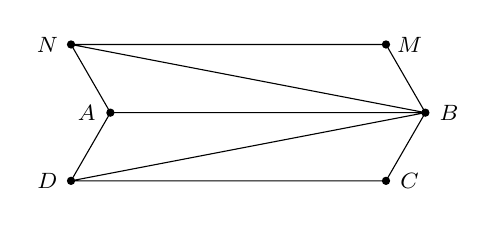
\begin{tikzpicture}[scale=1, font=\footnotesize, line join=round, line cap=round, >=stealth]
 				\path 
 				(0,0) coordinate (A)
 				(4,0) coordinate (B)
 				(A)+(120:1) coordinate (N)
 				(A)+(-120:1) coordinate (D)
 				(B)+(120:1) coordinate (M)
 				(B)+(-120:1) coordinate (C)
 				;
 				\draw (A)--(B)--(M)--(N)--cycle (A)--(D)--(C)--(B) (N)--(B)--(D);
 				\foreach \p/\r in {A/180,B/0,N/180,D/180,M/0,C/0}
 				\fill (\p) circle (1.5pt) node[shift={(\r:3mm)}]{$\p$};
 			\end{tikzpicture}
 		}
 	}
 \end{vd}
\subsubsection{Bài tập rèn luyện}
\subsubsection{Bài tập tự luận}
%%==========Bài 1
\begin{bt}%[Nguyễn Sĩ Đạt]%[1K4YB-2]
	\immini{Cho $E$ và $F$ lần lượt là trung điểm các cạnh $AB$ và $AC$ của tứ diện $ABCD$. Xác định vị trí tương đối của các đường thẳng $BC$, $AD$ và $EF$ với mặt phẳng $(BCD)$.}{
		\begin{tikzpicture}[scale=1, font=\footnotesize, line join=round, line cap=round, >=stealth]
			\path 
			(0,0) coordinate (B)
			(4,0) coordinate (D)
			(2,-1) coordinate (C)
			(B)+(2.5,3) coordinate (A)
			($(B)!.5!(A)$) coordinate (E)
			($(C)!.5!(A)$) coordinate (F)
			;
			
			\draw (A)--(B)--(C)--(D)--cycle (A)--(C) (E)--(F);
			\draw[dashed] (B)--(D);
			\foreach \p/\r in {A/90,B/180,D/0,C/-90,E/180,F/0}
			\fill (\p) circle (1.5pt) node[shift={(\r:3mm)}]{$\p$};
		\end{tikzpicture}
	}
	\loigiai{
		\begin{itemize}
			\item $BC$ có hai điểm chung $B$ và $C$ với $(BCD)$, suy ra $BC\subset (BCD)$.
			\item $AD$ có một điểm chung duy nhất $D$ với $(BCD)$, suy ra $AD$ cắt $(BCD)$ tại $D$.
			\item $EF$ là đường trung bình của tam giác $ABC$ suy ra $EF$ song song với $BC$.\\
			Giả sử $EF$ có điểm chung $O$ với $(BCD)$ thì $O$ thuộc giao tuyến $BC$ của hai mặt phẳng $(ABC)$ và $(BCD)$, suy ra $EF$ cắt $BC$ (mâu thuẫn với giả thiết $EF$ là đường trung bình). Vậy $EF\parallel (BCD)$.
		\end{itemize}
	}
\end{bt}
%%==========Bài 2
\begin{bt}%[Nguyễn Sĩ Đạt]%[1K4BB-2] 
	Cho hình chóp $S.ABCD$, đáy $ABCD$ là hình bình hành có $O$ là giao điểm hai đường chéo. Cho $M$ là trung điểm của $S C$. Chứng minh đường thẳng $O M$ song song với hai mặt phẳng $(S A D)$ và $(SAB)$.  
	\loigiai{	
	\immini{ Ta có $\heva{&OM\not\subset (SAD)\\&OM \parallel SA \,(\text{đường trung bình})\\&SA \subset (SAD)}\Rightarrow OM\parallel(SAD).$\\
	Ta có $\heva{&OM\not\subset (SAB)\\&OM \parallel SA \,(\text{đường trung bình})\\&SA \subset (SAB)}\Rightarrow OM\parallel(SAB).$ }
	{\begin{tikzpicture}[=>stealth,line join=round,line cap=round, font=\footnotesize, scale=.7]
	\def\a{6}
	\def\goc{230}
	\def\b{4}
	\def\h{5.5}
	\path
	(0,0)coordinate (A)++(0:\a)coordinate (B)++(\goc:\b)coordinate (C)++(180:\a)coordinate(D)
	($(A)!.5!(C)$)coordinate (O)
	(O)++(100:\h)coordinate (S)	
	($(S)!.5!(C)$)coordinate (M);
	\coordinate (K) at (-1.3,4);
%	\draw (-1.3,4)node[left]{$x$};
	\draw (S)--(B)--(C)--(D)--cycle (S)--(C) %(M)--(D) (D)--(K)
	;
	\draw[dashed] (O)--(S)--(A)--(C) (B)--(A)--(D)--(B) (M)--(O) 
	;
	\foreach \x/\g in{A/160,B/0,C/-90,S/90,O/-90,D/-90,M/10}
	\fill[black](\x)circle(1pt) ($(\x)+(\g:3.5mm)$)node{$\x$}
	;
	\end{tikzpicture}}	
	}	
\end{bt}
%%==========Bài 3
\begin{bt}%[Nguyễn Sĩ Đạt]%[1K4BB-2] 
	\immini{Cho hai điểm $A$, $B$ cùng thuộc mặt phẳng $(P)$ và một điểm $C$ không thuộc $(P)$. Vẽ đường thẳng $d_1$ đi qua $A$, $B$; $d_2$ đi qua $A$, $C$; $d_3$ đi qua $C$ và song song với $AB$ (hình bên). Tìm số điểm chung của mỗi đường thẳng vừa vẽ với $(P)$. Xét vị trí tương đối của mặt phẳng $(P)$ lần lượt đối với đường thẳng $d_1$, $d_2$, $d_3$.}{
		\begin{tikzpicture}[scale=1, font=\footnotesize, line join=round, line cap=round, >=stealth]
			\path
			(0,0) coordinate (A)
			(4,0) coordinate (B)
			(1,2) coordinate (D)
			($(B)+(D)-(A)$) coordinate (C)
			(2,3) coordinate (E)
			(3,-1) coordinate (F)
			(intersection of E--F and C--A) coordinate (M)
			(intersection of M--F and A--B) coordinate (N)
			(5,2.3) coordinate (G)
			(1,2.3) coordinate (H)
			(intersection of G--H and E--F) coordinate (K)
			;
			\draw (M)--+(0:1.8) (M)--+(180:1) node[above]{$d_1$};
			\draw[fill=black] 
			(M) node[above right]{$A$} circle (1pt) 
			(K) node[above right]{$C$} circle (1pt) 
			($(M)+(0:1.5)$) node[above]{$B$} circle (1pt)
			;
			\draw[dashed] (M)--(N);
			\draw($(F)!0.1!(M)$)node[above right]{$d_2$} (A)--(B)--(C)--(D)--cycle (E)--(M) (N)--(F) (G)--(H) ($(G)!.2!(H)$)node[above]{$d_3$};
			\draw    pic["$P$", draw=black, angle eccentricity=.7, angle radius=1cm]
			{angle=B--A--D}; %góc
		\end{tikzpicture}
	}
	\loigiai{
		Đường thẳng $d_1$ chứa hai điểm $A$, $B$ thuộc $(P)$, vậy $d_1\subset (P)$.\\
		Đường thẳng $d_2$ không nằm trong $(P)$ vì có chứa điểm $C$ không thuộc $(P)$. Mặt khác, $d_2$ lại có điểm $A$ chung với $(P)$, suy ra $d_2$ cắt $(P)$ tại $A$.
		Đường thẳng $d_3$ không nằm trong $(P)$ và song song với đường thẳng $d_1$ nằm trong $(P)$, suy ra $d_3\parallel (P)$.
	}
\end{bt}
%%==========Bài 4
\begin{bt}%[Nguyễn Sĩ Đạt]%[1K4KB-2] 
	Cho hai hình bình hành $ABCD$ và $ABEF$ không nằm trong cùng một mặt phẳng. Gọi $O$ và $O'$ lần lượt là tâm của $ABCD$ và $ABEF$. Chứng minh đường thẳng $O O'$ song song với các mặt phẳng $(CDFE)$, $(A D F)$ và $(B C E)$. 
	\loigiai{ 
	\immini{Ta có $\heva{&OO'\not\subset (CDFE)\\&OO'\parallel DF \\&DF\subset (CDFE)}\Rightarrow OO'\parallel (CDFE)$.\\
	Ta có $\heva{&OO'\not\subset (ADF)\\&OO'\parallel DF \\&DF\subset (ADF)}\Rightarrow OO'\parallel (ADF)$.\\
	Ta có $\heva{&OO'\not\subset (BCE)\\&OO'\parallel CE \\&CE\subset (BCE)}\Rightarrow OO'\parallel (BCE)$.}
	{\begin{tikzpicture}[=>stealth,line join=round,line cap=round, font=\footnotesize, scale=.9]	
	\coordinate (A) at (0,0);
	\coordinate (B) at (5,0); 
	\coordinate (C) at (4,-2);
	\coordinate (D) at (-1,-2);
	\coordinate (E) at (4,2);
	\coordinate (F) at (-1,2);
	\path	
	($(A)!.5!(F)$)coordinate (M)
	($(B)!.5!(E)$)coordinate (N)
	($(A)!.5!(D)$)coordinate (M1)
	($(B)!.5!(C)$)coordinate (N1);
	\draw (N1)node[above left]{$x$};
	\path (intersection of C--A and B--D)coordinate (O)
	(intersection of E--A and B--F)coordinate (O');
	\draw (B)--(C)--(D) (B)--(E)--(F) (D)--(F) (C)--(E) ;
	\draw[dashed] (M)--(N) (E)--(A)--(C) (F)--(B)--(D) (D)--(A)--(B) (F)--(A) (O)--(O') (M)--(O)--(N) (M1)--(N1);
	\foreach \x/\g in{A/180,B/0,C/0,D/180,E/0,F/180,O/-90,O'/90,M/180,N/0}
	\fill[black](\x)circle(1pt) ($(\x)+(\g:3mm)$)node{$\x$};
	%\draw (0.5,-3) node[right]{Hình 3};
	\end{tikzpicture}	} }	
\end{bt}
 

%%==========Bài 5
\begin{bt}%[Nguyễn Sĩ Đạt]%[1K4BB-2] 
	Cho tứ diện $ABCD$ và điểm $M$ thuộc cạnh $AB$. Gọi $(\alpha)$ là mặt phẳng qua $M$, song song với hai đường thẳng $B C$ và $AD$. Gọi $N$, $P$, $Q$ lần lượt là giao điểm của mặt phẳng $(\alpha)$ với các cạnh $AC$, $CD$ và $DB$.
	\begin{enumerate}
	\item Chứng minh $MNPQ$ là hình bình hành.
	\item Trong trường hợp nào thì $MNPQ$ là hình thoi?
	\end{enumerate}
	\loigiai{
	\immini{\begin{enumerate}
	\item Ta có $\heva{&MN \parallel BC\\&QP \parallel BC}\Rightarrow MN \parallel QP\quad (1).$\\
	Ta có $\heva{&NP \parallel AD\\&MQ \parallel AD}\Rightarrow NP \parallel MQ \quad (2).$\\
	Từ (1) và (2) suy ra tứ giác $MNPQ$ là hình bình hành.
	\item Để hình bình hành $MNPQ$ là hình thoi thì ta cần $MQ=PQ$.
	Để $MQ=PQ$ ta cần $M$ là trung điểm $AB$ và $AD=BC$.\\
	Vậy để $MNPQ$ là hình thoi ta cần bổ sung thêm $M$ là trung điểm $AB$ và $AD=BC$.
	\end{enumerate}}
	{\begin{tikzpicture}[=>stealth,line join=round,line cap=round, font=\footnotesize, scale=.7]
	\def\a{9}
	\def\goc{220}
	\def\b{5}
	\def\h{7.5}
	\path
	(0,0)coordinate (C)++(0:\a)coordinate (D)++(\goc:\b)coordinate (B)
	(C)++(50:\h)coordinate (A);
	\path
	($(A)!.6!(B)$)coordinate (M)
	($(A)!.6!(C)$)coordinate (N)
	($(D)!.6!(B)$)coordinate (Q)
	($(D)!.6!(C)$)coordinate (P);	
	\draw (A)--(C)--(B)--(D)--cycle (A)--(B) (N)--(M)--(Q);
	\draw[dashed] (D)--(C) (N)--(P)--(Q);
	\foreach \x/\g in{C/180,B/-90,D/0,A/90,M/20,N/140,Q/0,P/-90}
	\fill[black](\x)circle(1pt) ($(\x)+(\g:4mm)$)node{$\x$}
	;
	\end{tikzpicture}}	
	}	
\end{bt}

\centerline{\fcolorbox{red}{yellow!50}{\bf {CÂU HỎI TRẮC NGHIỆM (Tầm 10 - 20 câu theo theo tỉ lệ 4:3:2:1)}}}
\Opensolutionfile{ans}[ans/ans-1K1-3-Dang1]
%%==========Câu 1
\begin{ex}%[Nguyễn Sĩ Đạt]%[1K4BB-2]
Chọn khẳng định đúng trong các khẳng định sau
\choice
{Hai đường thẳng phân biệt cùng song song với một mặt phẳng thì song song nhau}
{\True Nếu $a\parallel (P)$ thì tồn tại trong $(P)$ đường thẳng $b$ để $b\parallel a$}
{Nếu $\heva{&a\parallel (P)\\&b \subset (P)}$ thì $a\parallel b$}
{Nếu $a\parallel (P)$ và đường thẳng $b$ cắt mặt phẳng $(P)$ thì hai đường thẳng $a$ và $b$ cắt nhau}
\loigiai{
Nếu $a\parallel (P)$ thì tồn tại trong $(P)$ đường thẳng $b$ để $b\parallel a$.
}
\end{ex}

%%==========Câu 2
\begin{ex}%[Nguyễn Sĩ Đạt]%[1K4YB-2]
Cho mặt phẳng $(\alpha)$ và đường thẳng $d \notin(\alpha)$. Khẳng định nào sau đây sai?
\choice
{Nếu $d \parallel (\alpha)$ thì trong $(\alpha)$ tồn tại đường thẳng $\Delta$ sao cho $\Delta \parallel  d$}
{\True Nếu $d \parallel (\alpha)$ và $b \subset(\alpha)$ thì $b \parallel  d$}
{Nếu $d \cap(\alpha)=\{A\}$ và $d' \subset(\alpha)$ thì $d$ và $d'$ hoặc cắt nhau hoặc chéo nhau}
{Nếu $d \parallel  c $; $ c \in(\alpha)$ thì $d \parallel (\alpha)$}
\loigiai{
Mệnh đề \lq\lq  Nếu $d \parallel (\alpha)$ và $b \subset(\alpha)$ thì $b \parallel  d$\rq\rq\ sai vì $b$ và $d$ có thể chéo nhau.
}
\end{ex}

%%==========Câu 3
\begin{ex}%[Nguyễn Sĩ Đạt]%[1K4YB-2]
Cho các mệnh đề:\\
1. $a \parallel  b, b \subset(P) \Rightarrow a \parallel (P)$.\\
2. $a \parallel (P), a \in(Q)$ với $\forall(Q)$ và $(Q) \cap(P)=b \Rightarrow b \parallel  a$.\\
3. Nếu hai mặt phẳng cắt nhau cùng song song với một đường thẳng thì giao tuyến của chúng cũng song song với đường thẳng đó.\\
4. Nếu $a$, $b$ là hai đường thẳng chéo nhau thì có vô số mặt phẳng chứa $a$ và song song với $b$. \\
Số mệnh đề đúng là:
\choice
{\True $3$}
{$1$}
{$2$}
{$4$}
\loigiai{
Mệnh đề \lq\lq  Nếu $a$, $b$ là hai đường thẳng chéo nhau thì có vô số mặt phẳng chứa $a$ và song song với $b$\rq\rq\ là mệnh đề sai vì nếu $a$, $b$ là hai đường thẳng chéo nhau thì chỉ có một mặt phẳng chứa $a$ và song song với $b$.
}
\end{ex}

%%==========Câu 4
\begin{ex}%[Nguyễn Sĩ Đạt]%[1K4YB-2]
Cho hai đương thằng $a$ và $b$ chéo nhau. Có bao nhiêu mặt phẳng chứa $a$ và song song với $b$?
\choice
{$3$}
{\True $1$}
{$2$}
{$4$}
\loigiai{
Nếu $a$, $b$ là hai đường thẳng chéo nhau thì chỉ có một mặt phẳng chứa $a$ và song song với $b$.
}
\end{ex}


%%==========Câu 5
\begin{ex}%[Nguyễn Sĩ Đạt]%[1K4YB-2]
	Cho hình chóp $S.ABCD$ có đáy $ABCD$ là hình bình hành. Đường thẳng $AD$ song song với mặt phẳng nào trong các mặt phẳng dưới đây?
	\choice
	{\True $(SBC)$}
	{$(ABCD)$}
	{$(SAC)$}
	{$(SAB)$}
	\loigiai{
	\immini
	{
	Do $AD \parallel BC$, $AD \not\subset (SBC) $ và $BC\subset (SBC)$ nên $AD\parallel (SBC).$
	}
	{
	\begin{tikzpicture}[scale=1, font=\footnotesize, line join=round, line cap=round, >=stealth]
	\def\bc{4} % cạnh BC
	\def\ba{2} % cạnh BA
	\def\h{4} % đường cao
	\def\gocB{30} % góc B của đáy
	\coordinate[label=below left:$B$] (B) at (0,0);
	\coordinate[label=above left:$A$] (A) at (\gocB:\ba);
	\coordinate[label=below:$C$] (C) at (\bc,0);
	\coordinate[label=right:$D$] (D) at ($(C)-(B)+(A)$);
	\coordinate[label=above:$S$] (S) at ($(A)+(90:\h)$);
	\draw (B)--(C)--(D)--(S)--cycle (S)--(C);
	\draw[dashed] (A)--(D) (S)--(A)--(B);
	\foreach \diem in {A,B,C,D,S}	\fill (\diem)circle(1.5pt);
	\newcommand{\gocv}[4][black]{\draw[#1] ($(#3)!5pt!(#2)$)--($(#3)!2!($($(#3)!5pt!(#2)$)!.5!($(#3)!5pt!(#4)$)$)$)--($(#3)!5pt!(#4)$);}
	\gocv{S}{A}{D}
	\end{tikzpicture}
	}	
	}
\end{ex}
%%==========Câu 6
\begin{ex}%[Nguyễn Sĩ Đạt]%[1K4BB-2]
	Cho hình chóp $S.ABCD$ có đáy là hình bình hành. Gọi $A'$, $B'$ lần lượt là trung điểm của $SA$, $SB$. Đường thẳng $A'B'$ song song với mặt phẳng nào sau đây?
	\choice
	{$(SAB)$}
	{$(SBC)$}
	{\True $(SCD)$}
	{$(SAD)$}
	\loigiai
	{
	\immini
	{
	Vì $A'B'$ song song với $AB$ và $AB$ song song với $CD$ nên $A'B'$ song song với $CD$. Hơn nữa, $A'B'$ không chứa trong $(SCD)$ nên $A'B'$ song song với $(SCD)$.
	}
	{
	\begin{tikzpicture}[scale=1, font=\footnotesize, line join=round, line cap=round, >=stealth]
	\def\bc{4} % cạnh BC
	\def\ba{2} % cạnh BA
	\def\h{4} % đường cao
	\def\gocB{30} % góc B của đáy
	\coordinate[label=below left:$B$] (B) at (0,0);
	\coordinate[label=above right:$A$] (A) at (\gocB:\ba);
	\coordinate[label=below:$C$] (C) at (\bc,0);
	\coordinate[label=right:$D$] (D) at ($(C)-(B)+(A)$);
	\coordinate (O) at ($(A)!.5!(C)$);
	\coordinate[label=above:$S$] (S) at ($(O)+(90:\h)$);
	\coordinate[label=right:$A'$] (A') at ($(A)!.5!(S)$);
	\coordinate[label=left:$B'$] (B') at ($(B)!.5!(S)$);
	\draw (B)--(C)--(D)--(S)--cycle (S)--(C);
	\draw[dashed] (A)--(D) (S)--(A)--(B) (A')--(B')
	;
	\foreach \diem in {A,B,C,D,S,A',B'}	\fill (\diem)circle(1.5pt);
	\end{tikzpicture}
	}
	}
\end{ex}
%%==========Câu 7
\begin{ex}%[Nguyễn Sĩ Đạt]%[1K4KB-2]
	Cho tứ diện $ABCD$. Gọi $G_1$, $G_2$ lần lượt là trọng tâm tam giác $BCD$ và $ACD$. Mệnh đề nào sau đây \textbf{sai}?	
	\choice
	{$ G_1G_2\parallel(ABD)$}
	{\True $ G_1G_2=\dfrac{2}{3}AB$}
	{$G_1G_2\parallel(ABC) $}
	{Ba đường thẳng $BG_1$, $AG_2$ và $CD$ đồng quy}
	\loigiai{\immini{Gọi $M$ là trung điểm của $CD$.\\
	Do $G_1$, $G_2$ lần lượt là trọng tâm tam giác $BCD$ và $ACD$ nên ta có \begin{center}
	$\dfrac{MG_1}{MB}=\dfrac{MG_2}{MC}=\dfrac{1}{3}\Rightarrow G_1G_2\parallel AB, \dfrac{G_1G_2}{AB}=\dfrac{1}{3}$.
	\end{center}
	Do $G_1G_2\parallel AB \Rightarrow G_1G_2\parallel (ABD)$ và $G_1G_2\parallel (ABC)$.\\
	Dễ thấy, ba đường thẳng $BG_1$, $AG_2$ và $CD$ đồng quy tại $M$.\\
	Vậy mệnh đề \lq\lq  $ G_1G_2=\dfrac{2}{3}AB$\rq\rq\ là mệnh đề \textbf{sai}. }{\begin{tikzpicture}[scale=.6,line join=round, line cap=round,smooth,font=\footnotesize,>=stealth]
	\coordinate (a) at (0,3);
	\coordinate (b) at (-3.36,0);
	\coordinate (c) at (-1,-2);
	\coordinate (d) at (4.28,0);
	\coordinate (m) at ($(d)!.5!(c)$);
	\coordinate (g1) at ($(b)!2/3!(m)$);
	\coordinate (g2) at ($(a)!2/3!(m)$);
	\draw (a)--(b)--(c)--(d)--cycle
	(m)--(a)--(c)
	;
	\draw[dashed] (d)--(b)--(m) (g1)--(g2) ;
	\fill (a)node[above]{$A$}circle(.06)
	(b)node[left]{$B$}circle(.06)
	(c)node[below]{$C$}circle(.06)
	(d)node[right]{$D$}circle(.06)
	(m)node[below right]{$M$}circle(.06)
	(g2)node[right]{$G_2$}circle(.06)
	(g1)node[below]{$G_1$}circle(.06);
	\end{tikzpicture}}
	}
\end{ex}

%%==========Câu 8
\begin{ex}%[Nguyễn Sĩ Đạt]%[1K4BB-2]
	Cho hai mặt phẳng $(\alpha);(\beta)$ cắt nhau và cùng song song với đường thẳng $d$. Khẳng định nào sau đây là đúng?	
	\choice
	{Giao tuyến của $(\alpha);(\beta)$ trùng với $d$}
	{Giao tuyến của $(\alpha);(\beta)$ song song hoặc trùng với $d$}
	{Giao tuyến của $(\alpha);(\beta)$ cắt $d$}
	{\True Giao tuyến của $(\alpha);(\beta)$ song song với $d$}
	\loigiai{Do $d$ không nằm trên mặt phẳng $(\alpha)$ và $(\beta)$ nên giao tuyến không thể trùng với $d$.\\
	Theo tính chất ta có giao tuyến song song với $d$.}
\end{ex}
%%==========Câu 9
\begin{ex}%[Nguyễn Sĩ Đạt]%[1K4KB-2]
 	Cho tứ diện $ABCD$. Gọi $G$ là trọng tâm tam giác $ABD$. $M$ là điểm trên cạnh $BC$ sao cho $MB=2MC$. Khi đó đường thẳng $MG$ song song với mặt phẳng nào dưới đây?
 	\choice
 	{\True $(ACD)$}
 	{$(BCD)$}
 	{$(ABD)$}
 	{$(ABC)$}
 	\loigiai{
 	\immini{
 	Gọi $E$ là trung điểm $AD$.\\
 	Xét tam giác $BCE$ có $\dfrac{BG}{BE}=\dfrac{BM}{BC}=\dfrac{2}{3}$ nên suy ra $MG\parallel(ACD)$.
 	}{
 	\begin{tikzpicture}[scale=1, font=\footnotesize, line join=round, line cap=round, >=stealth]
 	\def\ac{4} % cạnh AC
 	\def\ab{2} % cạnh AB
 	\def\as{4} % cạnh AS
 	\def\gocA{50} % góc A của đáy
 	\coordinate[label=left:$D$] (A) at (0,0);
 	\coordinate[label=right:$C$] (C) at (\ac,0);
 	\coordinate[label=below left:$B$] (B) at (-\gocA:\ab);
 	\coordinate[label=above:$A$] (S) at (70:\as);
 	\coordinate[label=below:$M$] (M) at ($(B)!2/3!(C)$);
 	\coordinate (N) at ($(A)!0.5!(B)$);
 	\coordinate[label=left:$G$] (G) at ($(S)!2/3!(N)$);
 	\coordinate[label=left:$E$] (E) at ($(S)!1/2!(A)$);
 	\draw (A)--(B)--(C)--(S)--cycle (S)--(B)--(E) (S)--(N);
 	\draw[dashed] (A)--(C)--(E) (M)--(G);
 	\foreach \diem in {A,B,C,S,N,G,M}\fill (\diem)circle(1.5pt);
 	\end{tikzpicture}
 	
 	}
 	}
 \end{ex} 

%%==========Câu 10
\begin{ex}%[Nguyễn Sĩ Đạt]%[1K4GB-2]
	Cho hình hộp $ABCD.A'B'C'D'$. Gọi $M$ là điểm trên cạnh $AC$ sao cho $AM=3MC$. Lấy $N$ trên cạnh $C'D$ sao cho $C'N=xC'D$. Với giá trị nào của $x$ thì $MN \parallel BD'$?
	\choice
	{\True $x=\dfrac{2}{3}$}
	{$x=\dfrac{1}{3}$}
	{$x=\dfrac{1}{4}$}
	{$x=\dfrac{1}{2}$}
	\loigiai{
	\immini{
	Từ giả thiết, ta có $M$ là trọng tâm tam giác $BCD$.\\
	Gọi $O$ và $I$ lần lượt là trung điểm của $AC$ và $DD'$. Khi đó, ta có $BD' \parallel (IAC)$.\\
	Trong $(CDD'C')$ gọi $N' = CI \cap C'D$, khi đó $N'$ là trọng tâm tam giác $CDD'$.\\
	Do đó $\dfrac{CM}{CO}=\dfrac{2}{3}=\dfrac{CN'}{CI} \Rightarrow MN' \parallel OI$. Mà $OI \parallel BD'$ nên $MN \parallel BD'$.\\
	Vậy $N' \equiv N$ và $x =\dfrac{2}{3}$.
	}{
	\begin{tikzpicture}[scale=1, font=\footnotesize, line join=round, line cap=round, >=stealth]
	\def\bc{4} % cạnh BC
	\def\ba{2} % cạnh BA
	\def\h{4} % đường cao
	\def\gocB{35} % góc B của đáy
	\coordinate[label=below left:$B$] (B) at (0,0);
	\coordinate[label=above right:$A$] (A) at (\gocB:\ba);
	\coordinate[label=below:$C$] (C) at (\bc,0);
	\coordinate[label=right:$D$] (D) at ($(C)-(B)+(A)$);
	\coordinate[label=above left:$A'$] (A') at ($(A)+(90:\h)$);
	\coordinate[label=left:$B'$] (B') at ($(B)-(A)+(A')$);
	\coordinate[label=above:$C'$] (C') at ($(C)-(A)+(A')$);
	\coordinate[label=right:$D'$] (D') at ($(D)-(A)+(A')$);
	\coordinate[label=above:$M$] (M) at ($(A)!3/4!(C)$);
	\coordinate[label=above right:$N$] (N) at ($(C')!2/3!(D)$);
	\draw (B')--(B)--(C)--(D)--(D')--(A')--(B')--(C')--(D') (C)--(C')--(D);
	\draw[dashed] (A')--(A)--(D) (C)--(A)--(B)--(D') (M)--(N);
	\foreach \diem in {A,B,C,D,A',B',C',D',M,N}	\fill (\diem)circle(1.5pt);
	\end{tikzpicture}
	}
	}
\end{ex}
\Closesolutionfile{ans}
\begin{indapan}{10}
	{ans/ans-1K1-3-Dang1}
\end{indapan}